%\section{شبیه‌سازی کانال رول استند در حضور کنترل‌کننده \lr{LQIDG}}\label{roll_lqidg_section_simulation}
%در بخش
%\ref{quadchanell_roll}
%شبیه‌سازی کانال رول استند چهارپره انجام شد.


 در این بخش به بررسی عملکرد چهارپره در حضور کنترل‌کننده \lr{LQIDG} پرداخته می‌شود. کنترل‌کننده \lr{LQIDG} در بخش
\ref{LQIDG}
بررسی شده‌است.
% در شبیه‌سازی برای بهینه‌سازی ضرایب وزنی \lr{LQIDG} از روش بهینه‌سازی
%\lr{TCACS} \cite{Karimi2010}
%استفاده شده‌است.
%تابع هزینه \lr{TCACS} به‌صورت
%\lr{ITSE}
%در نظر گرفته شده‌است. ضرایب وزنی خروجی بهینه‌سازی در پایین آورده شده‌است.
 در شبیه‌سازی برای بهینه‌سازی ضرایب وزنی مانند قسمت قبل عمل شده‌است.
\begin{equation}
	\boldsymbol{Q_{a_{LQIDG}}} = \begin{bmatrix}
		0.1707 &0& 0& 0\\
		0 &  0.12 & 0 &0 \\
		0 & 0 & 837.8606 & 0\\
		0 & 0 & 0 & 756.1341
	\end{bmatrix}, \quad R_{1_{LQDG}} =  1, \quad R_{2_{LQDG}} =  7.7422
\end{equation}
در گام بعد، با حل معادله
(\ref{coupled_riccatti_LQIDG})
(برای سادگی ماتریس‌های وزنی $\boldsymbol{{Q}_{a_2}}$ و $\boldsymbol{{Q}_{a_1}}$مساوی در نظر گرفته شده‌است)
ماتریس
$\boldsymbol{{K}_1}$
به‌صورت زیر به دست می‌آید.
\begin{equation}
	\boldsymbol{K_{a_1}} = \begin{bmatrix}
		10924.84&   39.83 & 1014.34 & -10629.93\\
		39.83   &  8.40 & 27.22& 11.70\\
		1014.34 &  27.22 & 1047.80 & -756.13\\
		-10658.93 & 11.70 & -756.13 & 10658.93
	\end{bmatrix}
\end{equation}
در نهایت فرمان کنترلی بهینه بازیکن اول از رابطه
(\ref{LQIDG_u})
به‌صورت زیر به دست می‌آید.
\begin{equation}
	u_1 = -\begin{bmatrix}
		28.1410 &   8.4017  & 27.2223  & 11.6894
	\end{bmatrix}\boldsymbol{x_{a}}(t)
\end{equation}

\begin{figure}[H]
	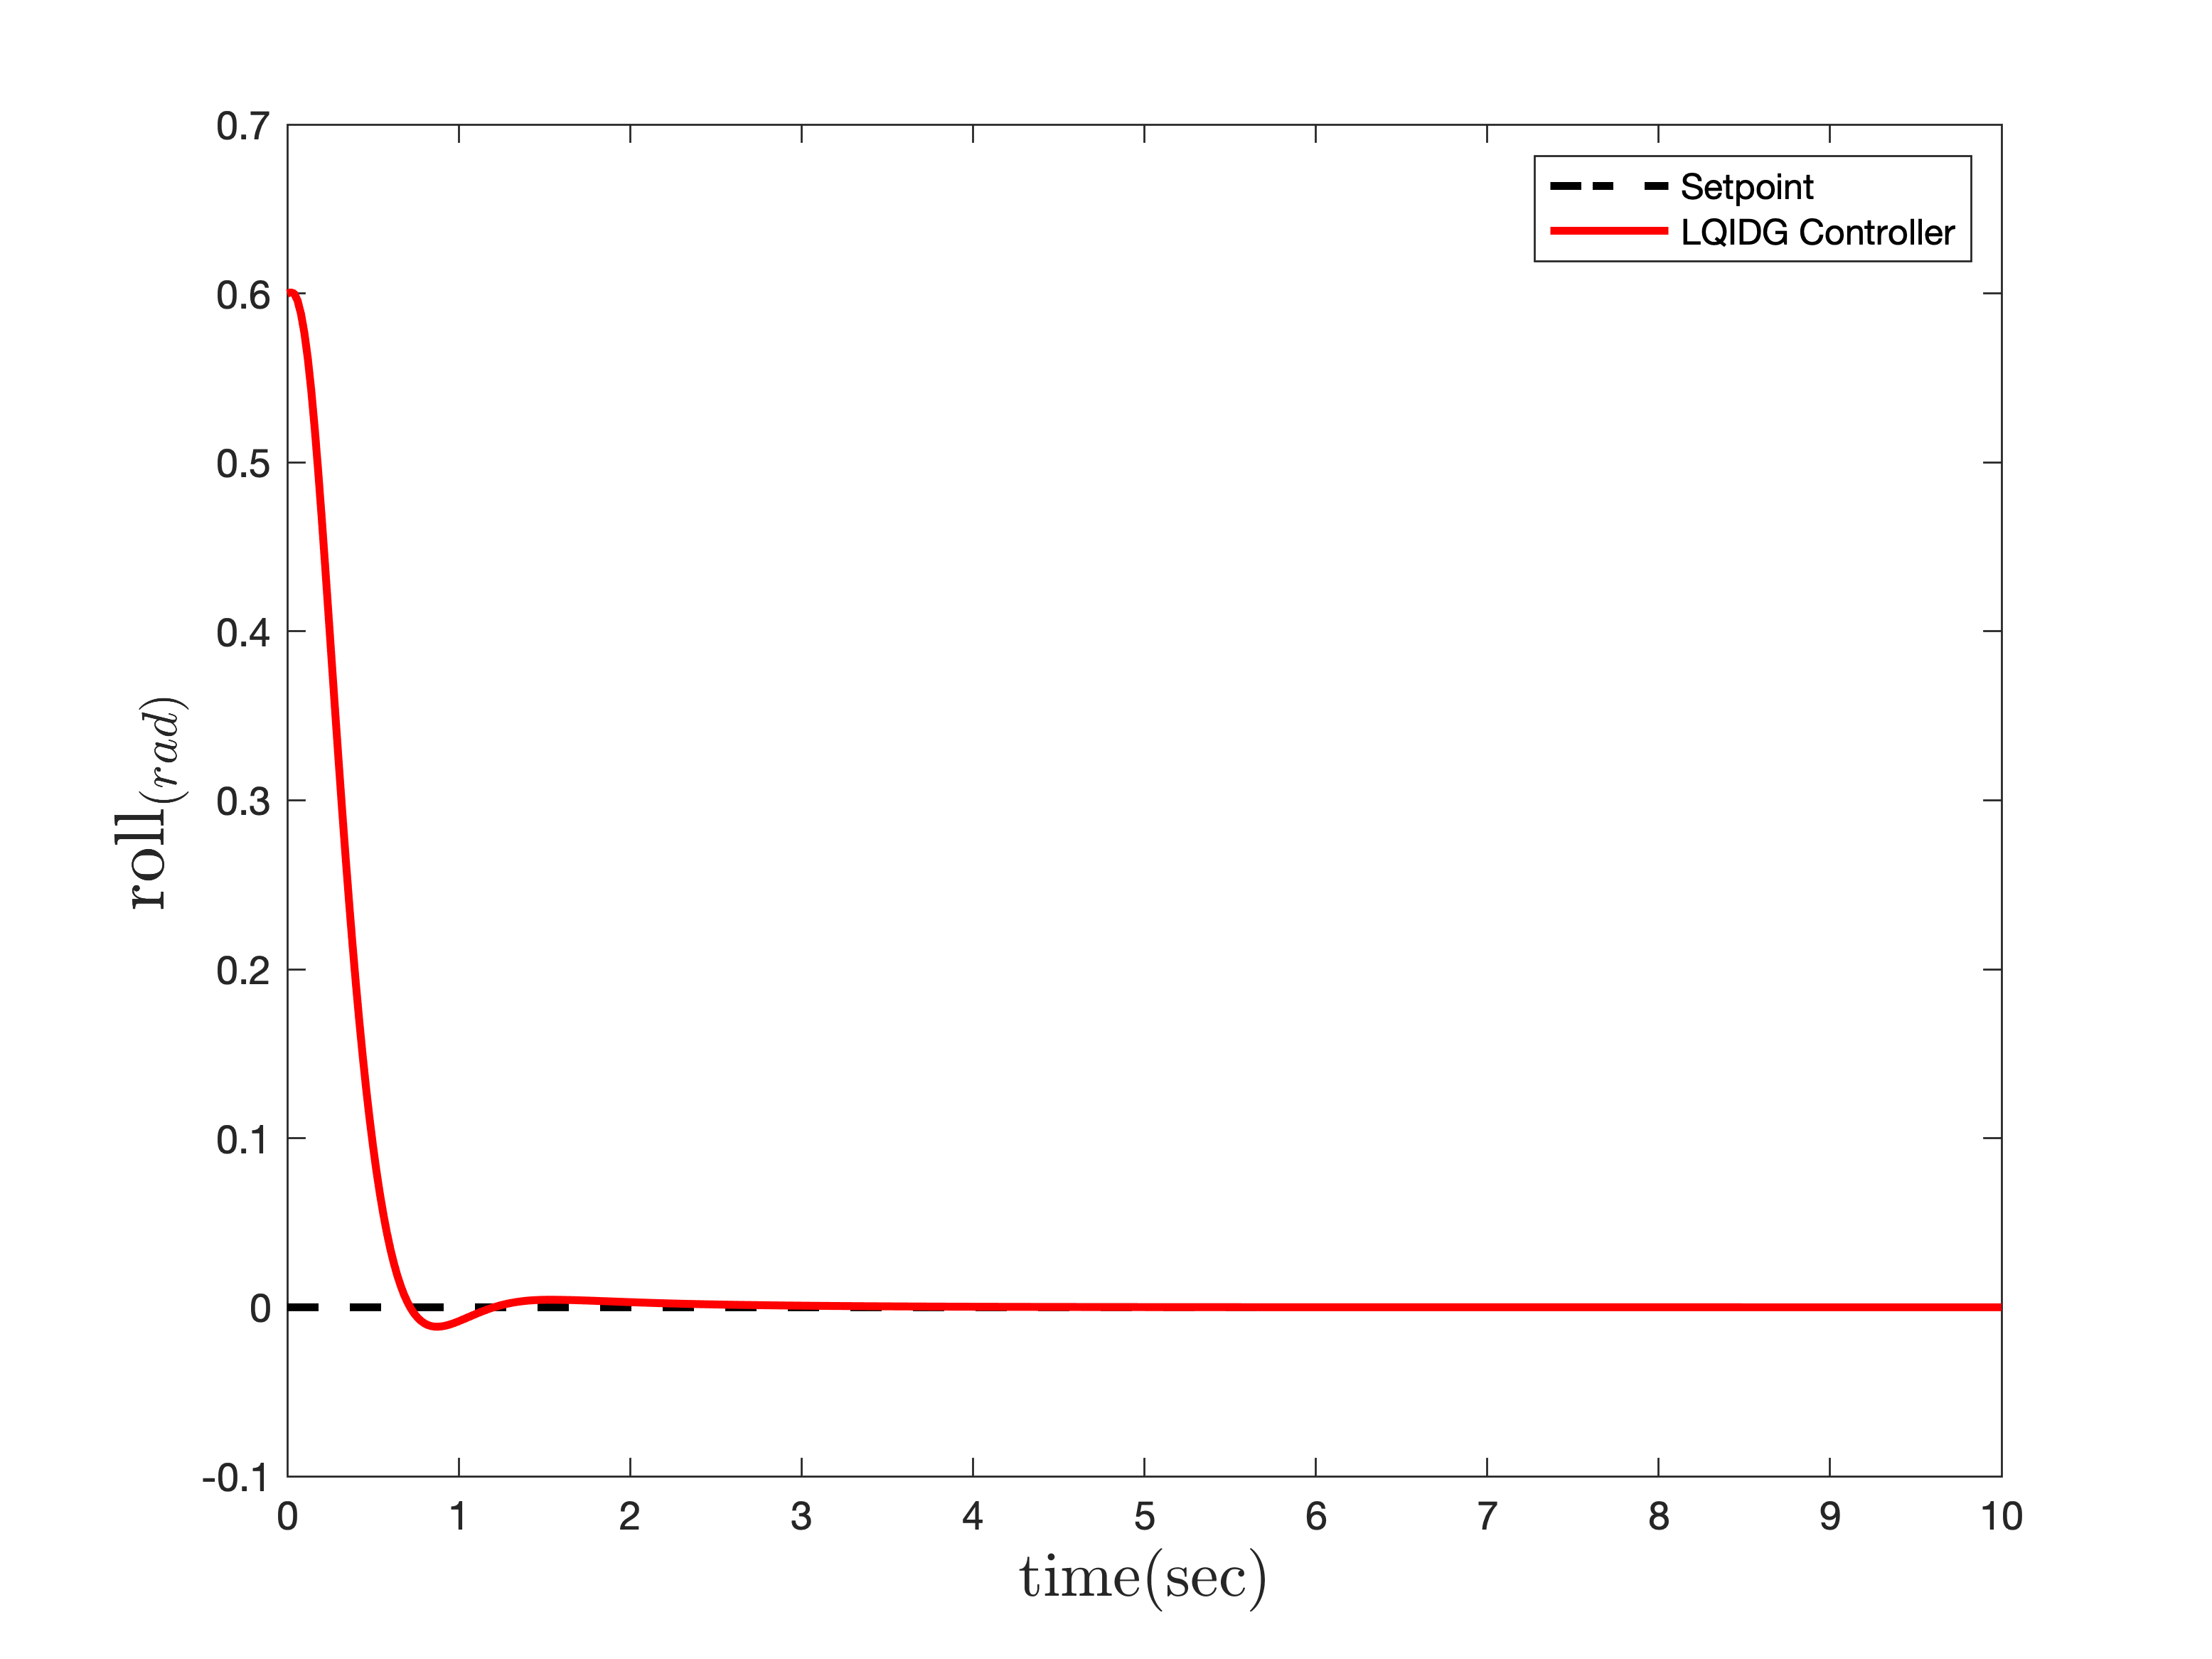
\includegraphics[width=.48\linewidth]{../Figures/MIL/LQIDG/Roll/lqidg_rollnn_.png}
	\centering
	\caption{عملكرد کنترل‌کننده \lr{LQIDG} در کنترل زاويه رول (تعقیب ورودی صفر)}
	\label{lqidg_roll_fig_simulation}
\end{figure}
\begin{figure}[H]
	\centering
	\subfigure[موتور شماره دو]{
		\centering
		\includegraphics[width=.45\linewidth]{../Figures/MIL/LQIDG/Roll/lqidg_roll_Omega_2nn_.png}
	}
	\subfigure[موتور شماره چهار]{
		\centering
		\includegraphics[width=.45\linewidth]{../Figures/MIL/LQIDG/Roll/lqidg_roll_Omega_4nn_.png}
	}
	\caption{‫‪فرمان کنترلی موتورهای دو و چهار در کنترل زاویه رول (تعقیب ورودی صفر)}
\end{figure}

\بدون‌تورفتگی همانطور که از شکل
\ref{lqidg_roll_fig_simulation}
مشخص است، زمان نشست در حدود یک ثانیه است و خطای ماندگار وجود ندارد.